\section{The one-sided contact process --- Proof of Theorem $1$}
\label{sec:contact}

\begin{quote}
{\small We review some results about the one-sided contact process and construct a link to a one-dependent oriented percolation model. We then exploit this link to obtain exponential bounds on the front propagation and survival times of the one-sided contact process. }
\end{quote}

\subsection{Classic results}

\begin{theorem}[{{\cite[Section 2.2]{liggett1977stochastic}}} and {{\cite[page 898, Claim III]{durrett1983supercritical}}}]\label{thm:upper_invariant}
If $(\eta_t)_{t \geq 0}$ is a one-sided contact process then $\Pr{\eta^\Z_t \in \cdot} \rightharpoonup \Pr{\eta^\Z_\infty \in \cdot} \eqdef \nu(\cdot)$ as $t \to \infty$ where $\nu$ is stationary, furthermore $\{ \eta^\Z_\infty (x) \}_{x \in \Z}$ is a stationary (shift) ergodic sequence. 
\end{theorem}

\begin{definition}
We call a one-sided contact process \textit{ergodic} if $\nu = \delta_{\{0\}}$ and \textit{nonergodic} otherwise. 
\end{definition}

\begin{remark}\label{rem:positive_density}
$\nu$ is sometimes called the \textit{upper invariant measure}. It is clear that $\nu$ is translation invariant, thus if we define $\rho \defeq \Pr{\nu(0) = 1}$ to be the probability that a given site is occupied under $\nu$, it follows that $\eta$ is ergodic if and only if $\rho = 0$. 
\end{remark}

\begin{lemma}\label{lem:old_results}
Let $\eta \defeq (\eta_t)_{t \geq 0}$ be a supercritical one-sided contact process. Then: 
\begin{enumerate}[(i)]
	\item $\eta$ is nonergodic
	\item For any $\Z \supseteq A \neq \varnothing$ it holds that $\Pr{\tau(\eta^A_t) = \infty} > 0$
	\item $\lim\limits_{M \rightarrow \infty} \sup\limits_{A \subseteq \Z: |A| = M} \Pr{\tau(\eta^A_t) = \infty} = 1$
	\item $\eta^\Z_t \geq \nu$ for all $t \geq 0$
	\item For all $\epsilon > 0$ and $M \in \N$, if $N$ is large enough then it holds that 
		\[\nu([0, N] \cap \cdot\text{ contains an interval of length $M$ }) > 1 - \epsilon. \]  
\end{enumerate}
\end{lemma}

\begin{proof}
The proof of (i) is given at \cite[page 902, top]{durrett1980growth}. For (ii) see \cite[Theorem 9.1]{harris1974contact} while (iii) can found in \cite[Lemma 5.2]{griffeath1979additive}. \\ 

To prove $(iv)$ consider the one-sided contact process $(\eta^\nu_t)_{t \geq 0}$ started from initial distribution $\nu$ constructed using $\scr{P}$. Note that since $\nu$ is stationary, $\eta^\nu_t \sim \nu$ for all $t \geq 0$. To conclude note that $\eta^\nu_0 \leq \eta^\Z_0 = \Z$ almost surely so that by attractivity $\eta^\nu_t \leq \eta^\Z_t$ for all $t \geq 0$ almost surely. \\

To prove $(v)$, let $\theta : \Omega \rightarrow \Omega$ be the left shift operator given by $\theta(\xi)(x) \defeq \xi(x + 1)$ and define $f : \Omega \rightarrow \{0, 1\}$ as $f(\xi) \defeq \mathbbm{1}_{\{\xi(1) = \xi(2) = ... = \xi(M) = 1\}}$. By Theorem \ref{thm:upper_invariant} $\theta$ is ergodic with respect to $\nu$ so that by Birkhoff's ergodic theorem it holds that 
\begin{equation} \label{eqn:birkhoff}
\frac{1}{N} \sum\limits^{N - 1}_{n = 0} f(\theta^n \eta^\Z_\infty) \xrightarrow[a.s.]{N \rightarrow \infty} \Ex{f(\eta^\Z_\infty)} = \nu(\, \cdot\, \supset \{1, ..., M\} ). 
\end{equation}
Once again consider the supercritical one-sided contact process $(\eta^\nu_t)_{t \geq 0}$ started from initial distribution $\nu$. By stationarity it follows that
\begin{align*}
\nu(\, \cdot\, \supset \{1, ..., M\}) &= \Pr{\eta^\nu_t \supset \{1, ..., M\}}                                    && \forall\, t \geq 0 \\
									  &\geq \Pr{\eta^\nu_0 (0) = 1 \text{ and } \eta^\nu_t \supset \{1, ..., M\}} && \forall\, t \geq 0. 
\end{align*}

Define $G(M, t)$ to be the event that in the time interval $[0, t]$ there are exactly $M$ clockrings when restricted to sites in $[0, M]$ and they satisfy $0 \leq T_{1, 1} < T_{2, 1} < ... < T_{M, 1} \leq t$. By basic properties of the exponential distribution for $t > 0$ we have
\begin{equation}\nonumber
\Pr{G(M, t)} > 0. 
\end{equation}
With this we can show that $\Ex{f(\eta^\Z_\infty)} > 0$: 
\begin{align*}
\Pr{\eta^\nu_0 (0) = 1 \text{ and } \eta^\nu_t \supset \{1, ..., M\}} &\geq \PrCond{\eta^\nu_t \supset \{1, ..., M\}}{\{\eta^\nu_0 (0) = 1\} \cap G(M, t)} \\ 
&\qquad \times \Pr{\eta^\nu_0 (0) = 1} \Pr{G(M, t)} \\
&\geq p^M \Pr{\eta^\nu_0 (0) = 1} \Pr{G(M, t)}. 
\end{align*}
Since $(\eta^\nu_t)_{t \geq 0}$ is supercritical $\rho = \Pr{\eta^\nu_0 (0) = 1} > 0$ by part (i) and Remark \ref{rem:positive_density}. By (\ref{eqn:birkhoff}) it follows that $\eta^\Z_\infty$ contains an interval of length $M$ almost surely infinitely many times. Thus we can choose $N$ large enough such that $\eta^\Z_\infty \cap [-N, N]$ contains an interval of length $M$ with probability greater than $1 - \epsilon$. By translation invariance the same holds for $\eta^\Z_\infty \cap [0, 2N]$ and the result follows. 
\end{proof}

\begin{definition}
Let $\eta \defeq (\eta_t)_{t \geq 0}$ be a one-sided contact process. For $A \subseteq \Z$ define $r^A_t \defeq \sup\eta^A_t$ and $l^A_t \defeq \inf\eta^A_t$ to be the right and left edge processes of $(\eta^A_t)_{t \geq 0}$. 
\end{definition}
\begin{remark}
Note that by definition $r^A_t = X(\eta^A_t)$ however the former notation is more convenient for what follows. 
\end{remark}

\begin{theorem}[{{\cite[page 6 (c)]{durrett1983supercritical}}}]\label{thm:convergence}
Let $(\eta_t)_{t \geq 0}$ be a supercritical one-sided contact process. Then there exist constants $0 \leq \beta < \alpha$ such that for all $|A| < \infty$, on $\{\tau(\eta^A_\cdot) = \infty\}$ it holds that
\begin{equation}\nonumber
\frac{r^A_t}{t} \xrightarrow[a.s.]{t \rightarrow \infty} \alpha \hspace{5mm} \text{and} \hspace{5mm} \frac{l^A_t}{t} \xrightarrow[a.s.]{t \rightarrow \infty} \beta.
\end{equation}
\end{theorem}

\subsection{Percolation construction}

\begin{figure}[!h]
  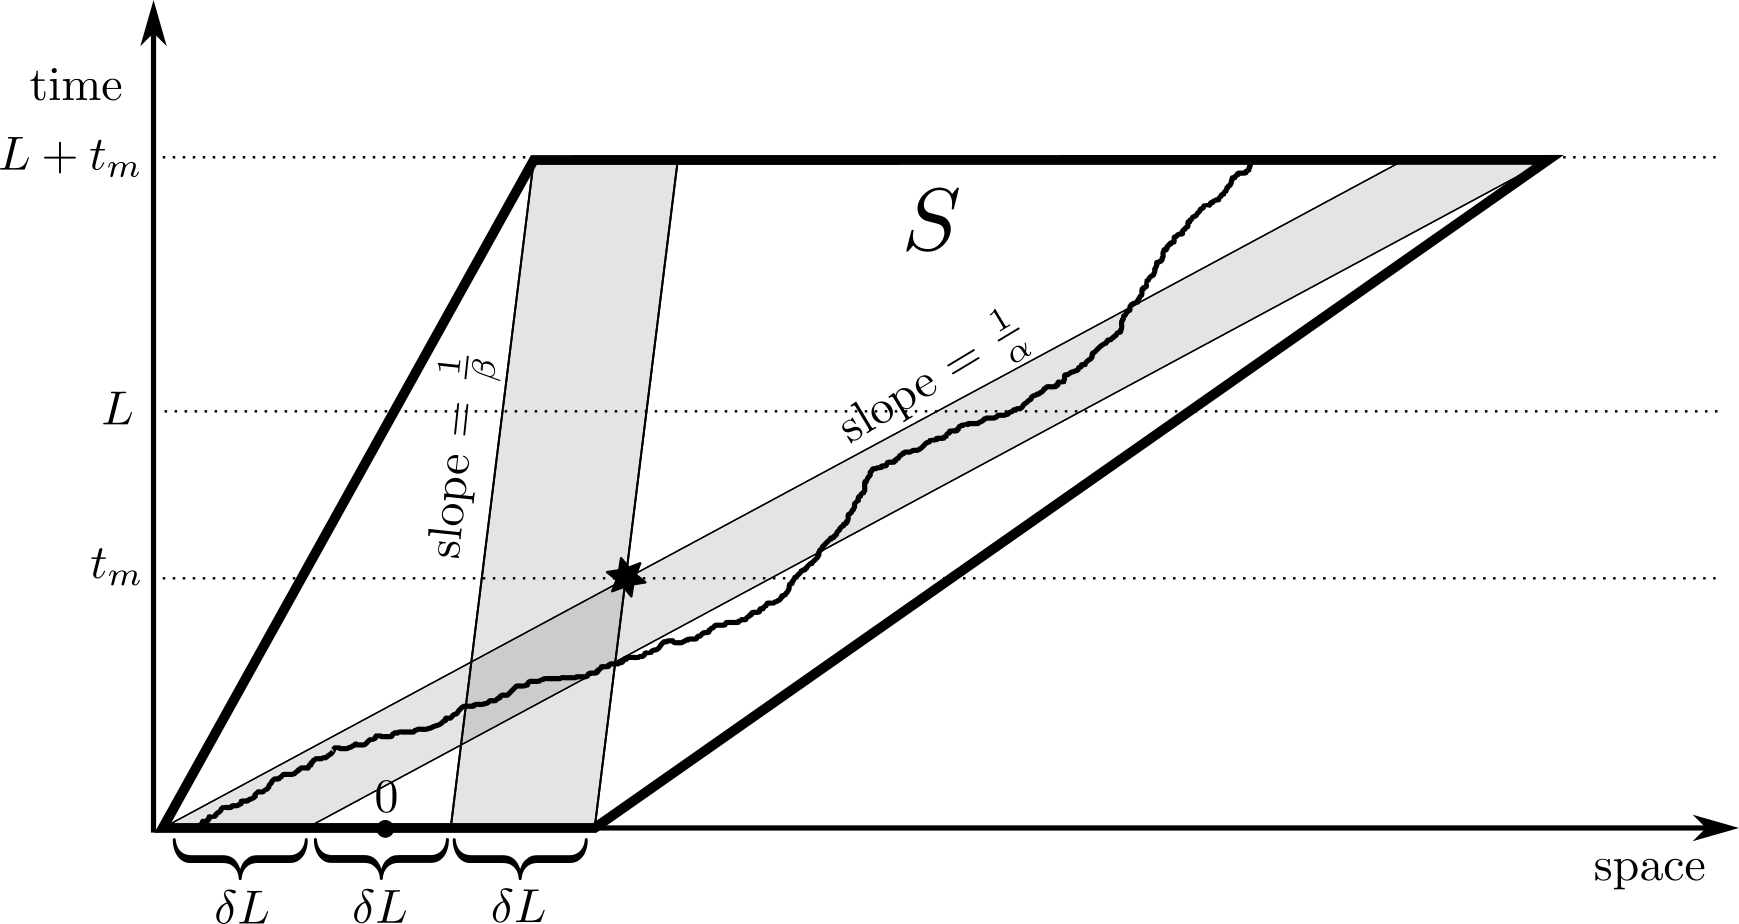
\includegraphics[width=\linewidth]{images/construction_single_tile}
  \caption{A visualisation of $S$ and a right nice path. }
  \label{fig:construction_single_tile}
\end{figure}

\begin{definition}
A \textit{path} in the graphical representation $\scr{P}$ connecting space-time points $(x, t), (y, s)$ with $t \leq s$ is a set of points $\{(z(r), r)\}_{r \in [t,s]} \subset \Z \times \R_{\geq 0}$ parametrised by $r \in [t, s]$ such that 
\begin{enumerate}[(i)] 
\item $z(t) = x$ and $z(s) = y$
\item No recovery occurs in $\{(z(r), r)\}_{r \in [t,s]} \subset \scr{P}$
\item The trajectory follows arrows i.e. $z(r-) \neq z(r)$ only if there is an arrow from $z(r-)$ to $z(r)$ at time $r$.   
\end{enumerate}
\end{definition}

Let $\delta > 0$ be a constant and $S$ be the convex quadrilateral defined by the four vertices $\{(- \frac{3 \delta L}{2}, 0), (\frac{3 \delta L}{2}, 0), (\beta (L + t_m) + \frac{3 \delta L}{2}, L + t_m), (\alpha (L + t_M) - \frac{3 \delta L}{2}, L + t_m) \}$, see Figure \ref{fig:construction_single_tile} for reference. Let $t_m = \frac{3\delta L }{\alpha - \beta}$ and define R to be the event that a \textit{right nice path} exists, which is a path inside $S$ that starts from $(- \frac{3 \delta L}{2}, - \delta L) \times \{0\}$ goes through $(\alpha t_m - \frac{ 3 \delta L }{2}, \infty) \times \{t_m\}$ and through $(\alpha L - \frac{3 \delta L}{2},\alpha L - \frac{\delta L}{2}) \times \{L\}$ and reaches $\Z \times \{ L + t_m \}$. In other words, looking at Figure \ref{fig:construction_single_tile}, a path inside $S$ that starts from $(- \frac{3 \delta L}{2}, - \delta L) \times \{0\}$, falls to the right of the star at time $t_m$, falls inside the right gray-shaded region at time $L$ and survives until time $L + t_m$. The star lies at the last intersection of the two shaded areas, which is easily checked to occur at time $t_m$. We always take $\delta < \frac{(\alpha - \beta)}{3}$ so that $t_m < L$. Analogously, for the left side define \textit{left nice paths} and the event $H$ that one occurs. Finally, let $E \defeq R \cap H$ be the event that both left and right nice paths exist. \\

\begin{lemma}\label{lem:construction}
For fixed $\frac{\alpha - \beta}{3} > \delta$ and $\epsilon > 0$ we can take $L$ large enough such that $R$ happens with probability greater than $1 - \epsilon$.  
\end{lemma}

\begin{remark}
From here on in this section `with high probability' is equivalent to `with probability greater than $1 - k \epsilon$' for some integer $k$ independent of $\epsilon$. We will sometimes abbreviate `with high probability' to `w.h.p.'.  
\end{remark}

\begin{proof}
Let $I_\delta = \left( \frac{ - 3 \delta L}{2}, - \delta L \right)$. By Lemma \ref{lem:old_results} part $(iii)$ we may take $L$ large enough so that $(\eta^{I_\delta}_t)_{t \geq 0}$ survives with high probability - call this threshold $L'$. As a consequence of almost sure convergence of the velocity of the edge processes, we can take $L$ large enough such that $(r^{I_\delta}_t)_{t \geq 0}$ goes through $(\alpha t_m  - \frac{5 \delta L }{4}, \infty) \times \{t_m\}$ and through $(\alpha L - \frac{5 \delta L}{4}, \alpha L + \frac{\delta L}{2}) \times \{L\}$ with high probability. Similarly for the left edge process, for large enough $L$ we have $l^{- I_\delta}_{t_m} < \alpha t_m - \frac{3 \delta L}{2}$ w.h.p. so that $l^{- I_\delta}_t$ and $r^{I_\delta}_t$ cross before time $t_m$. Note that the left and right edge processes are not paths, however there is a path to all points $(r^{I_\delta}_t, t)$ and $(l^{I_\delta}_t, t)$ from $I_\delta \times \{0\}$ and $-I_\delta \times \{0\}$ respectively. Define $s_t \defeq \sup\{x \in \eta^{I_\delta}_t \mid\ \exists \text{ path from } (x, t) \text{ to } \Z \times \{L + t_m \} \}$ so that $\{(s_t, t)\}_{0 \leq t \leq L + t_m}$ is the rightmost path connecting $I_\delta \times \{0\}$ with $\Z \times \{L + t_m\}$. We will show that the path $(s_t)_{t \geq 0}$ is a right nice path with high probability. \\

\begin{figure}[!h]
  \includegraphics[width=\linewidth]{images/construction_right}
  \caption{An example realisation of the edge processes. In red we see the path from $\Z \times \{0\}$ through the $\sfrac{\delta}{4}$-width `gate' surviving up until $\Z \times \{L + t_m\}$ }
  \label{fig:construction_right}
\end{figure}

By definition $s_t \leq r^{I_\delta}_t$ for all $0 \leq t \leq L + t_m$ so that in particular $s_L \leq r^{I_\delta}_L < \alpha L - \frac{\delta L}{2}$ w.h.p.. What remains to be shown is $\{(s_t, t)\}_{0 \leq t \leq L + t_m} \subset S$  and that $s_{t_m} > \alpha t_m - \frac{3 \delta L }{2}$ and $s_L > \alpha L - \frac{3 \delta L}{2}$ w.h.p.. We postpone showing inclusion in $S$ to the end of the proof. For the first of the other two claims take $L$ large enough such that $N = \frac{\delta L}{4}$ satisfies Lemma \ref{lem:old_results} part $(v)$ with $M = L'$. By part $(iv)$ of the same Lemma this implies that $\eta^\Z_{t_m} \cap (\alpha t_m - \frac{3 \delta L}{2}, \alpha t_m - \frac{5 \delta L}{4})$ contains an interval of length $L'$ with high probability. By the definition of $L'$ this implies that with high probability there is a path from $\Z \times \{0\}$ through $(\alpha t_m - \frac{3 \delta L}{2}, \alpha t_m - \frac{5 \delta L}{4}) \times \{t_m\}$ up to $\Z \times \{ L + t_m \}$; call this path $(w_t)_{t \geq 0}$. Now, using the edge processes $(r^{I_\delta}_t)_{t \geq 0}$, $(l^{- I_\delta}_t)_{t \geq 0}$ and the path just constructed we can create a new path from $I_\delta \times \{ 0 \}$ through $(\alpha t_m - \frac{ 3 \delta L}{2}, \alpha t_m - \frac{5 \delta L}{4}) \times \{t_m\}$ up to $\Z \times \{ L + t_m \}$. To do this let $\{(r_t, t)\}_{0 \leq t \leq t_m}$ and $\{(l_t, t)\}_{0 \leq t \leq t_m}$ be the paths connecting $I_\delta \times \{0\}$ and $-I_\delta \times \{0\}$ to $(r^{I_\delta}_{t_m}, t_m)$ and $(l^{-I_\delta}_{t_m}, t_m)$ respectively. Since $l^{-I_\delta}_{t_m} < r^{I_\delta}_{t_m}$ the two paths must cross before time $t_m$. Finally observe that at least one of $(l_t)_{t \leq t_m}$ and $(r_t)_{t \leq t_m}$ must cross the path $(w_t)_{t \geq 0}$. Hence we can always concatenate segments of $(l_t)_{t \leq t_m}$, $(r_t)_{t \leq t_m}$ and $(w_t)_{t \geq 0}$ to get the required path from $I_\delta \times \{0\}$ through $(\alpha t_m - \frac{ 3 \delta L}{2}, \alpha t_m - \frac{5 \delta L}{4}) \times \{t_m\}$ up to $\Z \times \{ L + t_m \}$. This proves in particular that $s_{t_m} > \alpha t_m - \frac{3 \delta L }{2}$. The claim $s_L > \alpha L - \frac{3 \delta L}{2}$ follows by an analogous argument. \\

To show that $\{(s_t, t)\}_{0 \leq t \leq L + t_m} \subset S$ w.h.p. first note that on the high probability event $\{ \tau(\eta^{I_\delta}_\cdot) = \infty\}$ it holds for all $t \geq 0$ that $r^{I_\delta}_t = r^{(- \infty, - \delta L]}_t$. Thus on $\cal{G} \defeq \{ \tau(\eta^{I_\delta}_\cdot) = \infty\}$ by translation invariance we may write for all $t_0 \geq 0$
\begin{flalign*}
& \PrCond{\left|r^{I_\delta}_t - (\alpha t - \delta L)\right| < \frac{\delta L}{2},\ \forall\, t \in [t_0, L + t_m]}{\cal{G}} &\\
& \quad = \PrCond{\left|r^{(- \infty, - \delta L]}_t - (\alpha t - \delta L)\right| < \frac{\delta L}{2},\ \forall\, t \in [t_0, L + t_m]}{\cal{G}}  &\\
& \quad = \PrCond{\left|\frac{r^{(- \infty, 0]}_t}{t} - \alpha \right| < \frac{\delta L}{2t},\ \forall\, t \in [t_0, L + t_m]}{\cal{G}} 
\geq \PrCond{\left|\frac{r^{(- \infty, 0]}_t}{t} - \alpha \right| < \frac{\delta}{4},\ \forall\, t \geq t_0}{\cal{G}} &\\
\end{flalign*}
Now simply take $t_0$ large enough such that the above probability is high. Note that $t_0$ only depends on $\epsilon$ and $\delta$. What this equation says is that with high probability, for all times after $t_0$ the right edge process started from $I_\delta$ falls inside the gray $\sfrac{\delta L}{2}$-tube as seen on Figure \ref{fig:construction_single_tile}, assuming that $L$ is large enough such that $\sfrac{\delta L}{2} \geq 1$. By the same argument on the event $\cal{G}$
\begin{equation}\nonumber
\left. \sup\limits_{0 \leq t \leq t_0} \left| r^{I_\delta}_t - (\alpha t - \delta L) \right|\right|\cal{G} \sim \left.\sup\limits_{0 \leq t \leq t_0} \left| r^{(- \infty, 0]}_t - \alpha t \right|\right|\cal{G} \eqdef X. 
\end{equation}
Since $X < \infty$ almost surely, we can take $L$ large enough so that $X < \delta L$ with high probability. With this we can conclude the proof that $\{(s_t, t)\}_{0 \leq t \leq L + t_m} \subset S$ w.h.p.. \\

Combining all our estimates during this proof gives the conclusion. 
\end{proof}

\begin{corollary}
For fixed $\frac{\alpha - \beta}{3} > \delta$ and $\epsilon > 0$ we can take $L$ large enough such that $E$ occurs with probability greater than $1 - \epsilon$. 
\end{corollary}

\begin{proof}
We saw $R$ occurs w.h.p.. An analogous argument shows that $H$ occurs w.h.p.. This implies that $E = R \cap H$ occurs with high probability. 
\end{proof}

\begin{definition}[Oriented percolation]
Let $U \defeq \{ (j, k) \in \Z \times \Z_{\geq 0} \mid j + k \equiv 0\ (\text{mod } 2)\}$ with the norm $\Vert(j,k)\Vert \defeq \frac{|j| + |k|}{2}$. A \textit{1-dependent oriented percolation model $\Lambda$ with density $\rho$ on $U$} is a collection of $\{0,1\}$-valued random variables $\{\Lambda(j,k)\}_{(j,k) \in U}$ such that $\Pr{\Lambda(j,k) = 1} = \rho$ and if $I \subset U$ contains no nearest neighbours then $\{\Lambda(j,k)\}_{(j,k) \in I}$ are independent. A \textit{path} in $\Lambda$ is a sequence $(j_1,k_1), ..., (j_n, k_n)$ in $U$ which satisfies $k_{l+1} = k_l + 1$ and $j_{l+1} = j_l \pm 1$ for all $l = 1, 2, ..., n - 1$. The path is said to be active if $\Lambda(j,k) = 1$ for each $l = 1,2,...,n$. Percolation from $(0,0)$ is said to occur if there is an active infinite path starting from $(0,0)$. 
\end{definition}

Define the grid of points $\{c_{j, k} \}_{(j, k) \in U}$ as
\[
c_{j, k} \defeq \left(c^{(1)}_{j,k}, c^{(2)}_{j,k}\right) = \left( \left[ \frac{k + j}{2}(\alpha - \delta) + \frac{k - j}{2}(\beta + \delta) \right] L, k L\right). 
\]
Now let $S_{j,k} \defeq S + c_{j,k}$ for $(j,k) \in U$ and $\{R_{j,k}\}_{(j,k)\in U}, \{H_{j,k}\}_{(j,k) \in U}$ be the events that right and left nice paths exist in the translated graphical representation $\scr{P} - c_{j,k}$, futhermore define $E_{j,k} \defeq R_{j,k} \cap H_{j,k}$. 

\begin{theorem}\label{thm:percolation}
There exists $\delta < \frac{\alpha - \beta}{3}$ such that for large enough $L$ the collection of random variables $\{\mathbbm{1}_{E_{j,k}}\}_{(j,k) \in U}$ is a one-dependent oriented percolation model on $U$ such that the density goes to $1$ as $L$ goes to infinity. 
\end{theorem}

\begin{figure}[!h]
  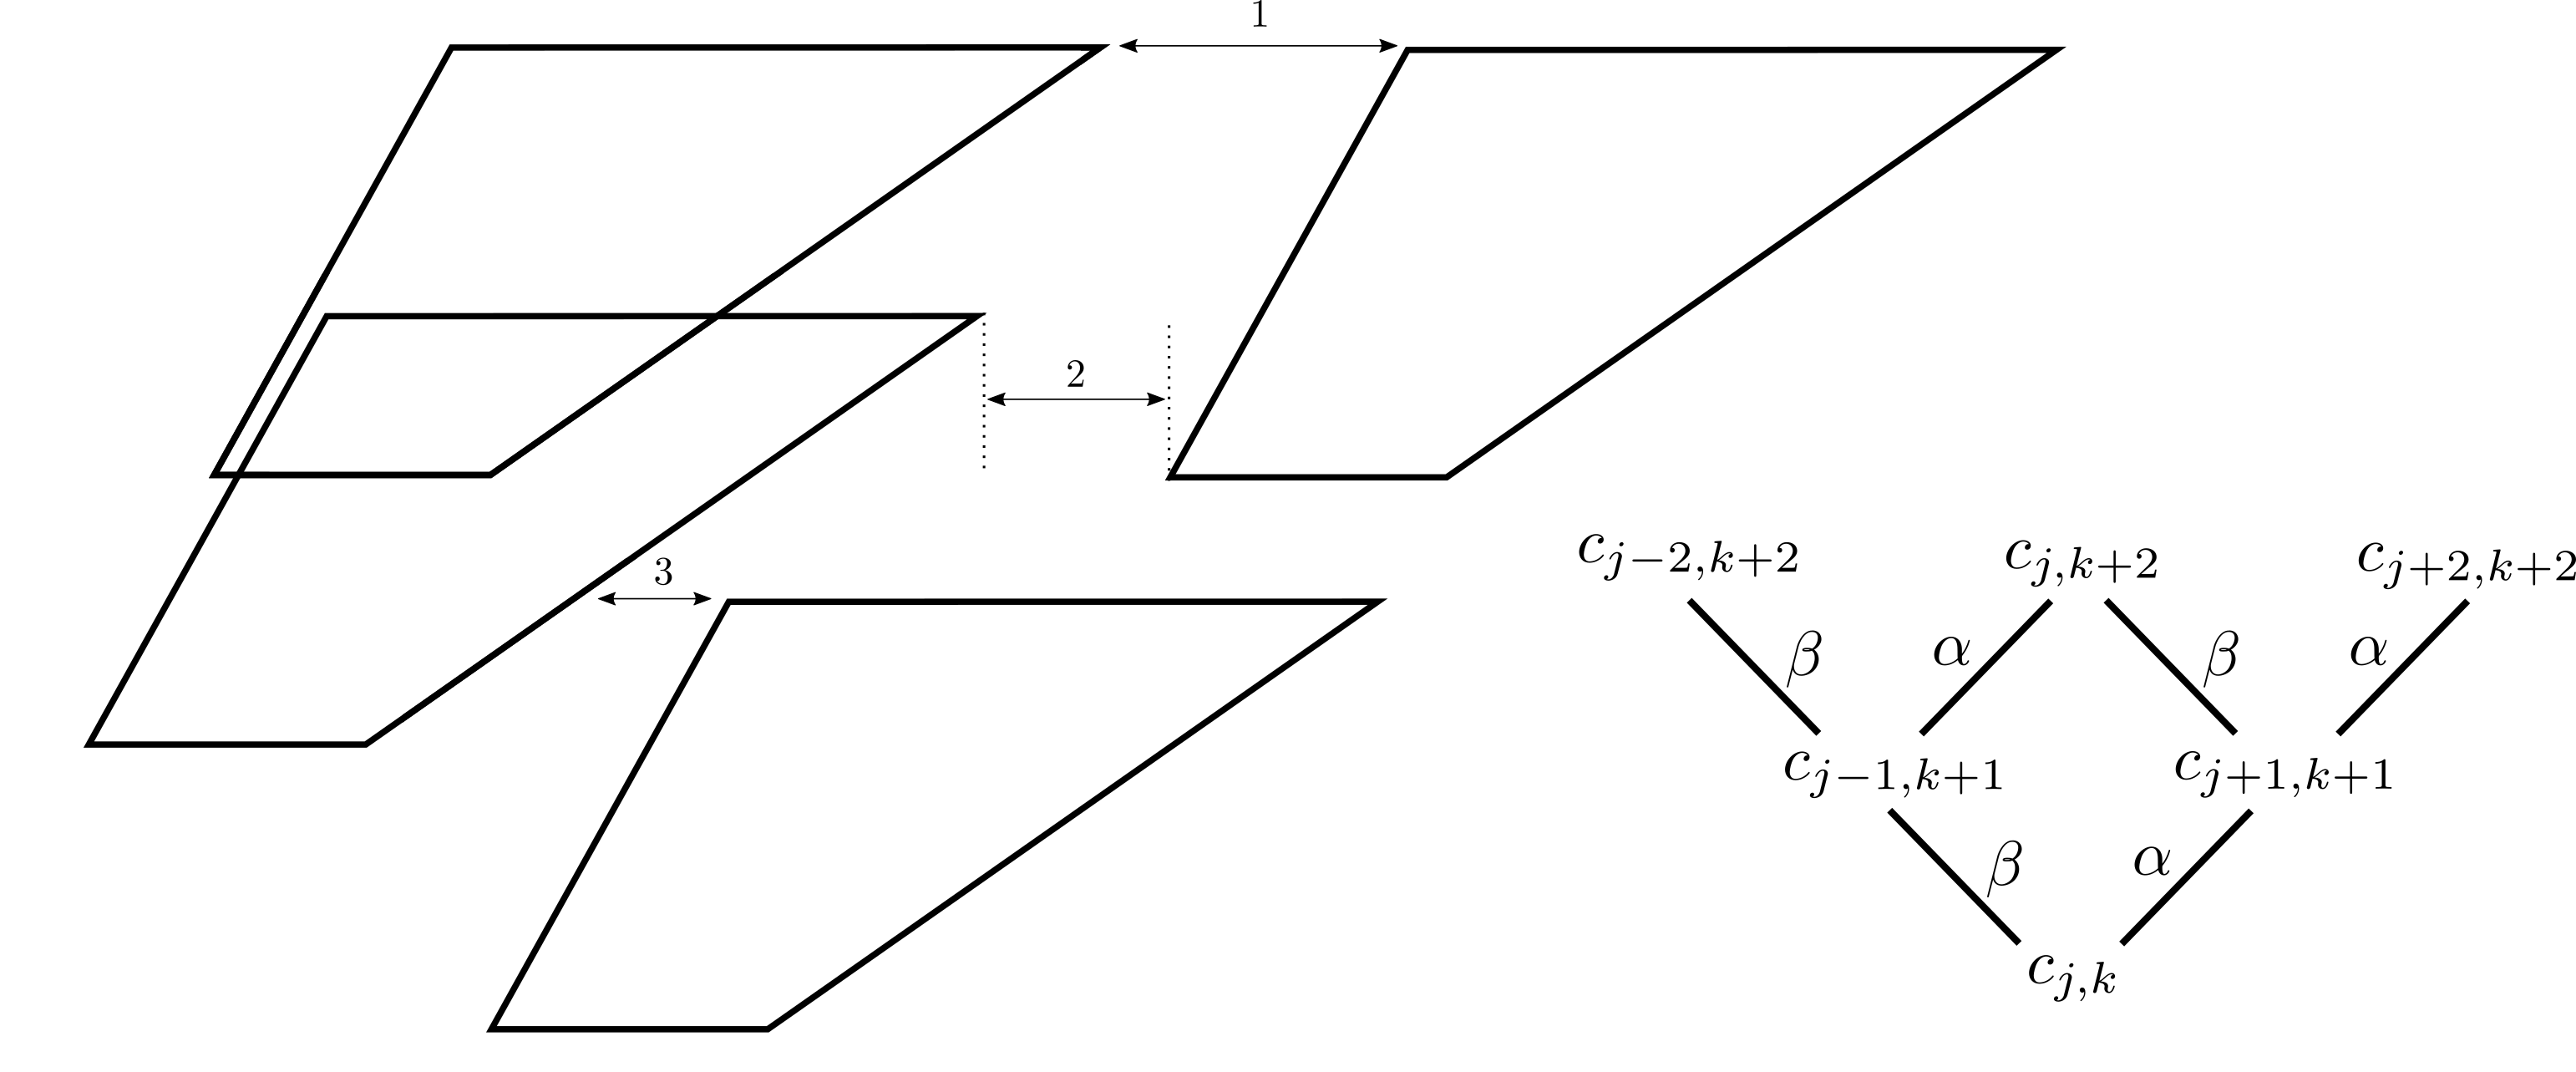
\includegraphics[width=\linewidth]{images/construction_intersections}
  \caption{The three different distances that we show are positive in the proof of Lemma \ref{lem:dependency}. }
  \label{fig:construction_intersections}
\end{figure}
\begin{lemma}\label{lem:dependency}
Independent of $L$ we can take $\delta$ small enough such that two quadrilaterals $S_{j_1,k_1}, S_{j_2, k_2}$ intersect only if $(j_1, k_1), (j_2, k_2)$ are nearest neighbours in $U$. 
\end{lemma}

\begin{proof}
Notice that both space and time are scaled by $L$ so that we may set $L = 1$ without loss of generality. Take $(j,k) \in U$. Recall that we asserted $t_m = \frac{3\delta}{\alpha - \beta} < 1$ so that quadrilaterals two or more rows apart cannot intersect. Thus it is sufficient to show that $S_{j, k} \cap S_{j - 4, k} = S_{j,k} \cap S_{j + 3, k + 1} = S_{j,k} \cap S_{j - 3, k + 1} = \varnothing$ for small enough $\delta$. For a visualisation see Figure \ref{fig:construction_intersections}. Note that the space-coordinate of $c_{j,k}$ satisfies the recursive equations

\begin{equation}\nonumber
c^{(1)}_{j,k} = c^{(1)}_{j - 1, k - 1} + \alpha L + \cal{O}(\delta L) = c^{(1)}_{j + 1, k - 1} + \beta L + \cal{O}(\delta L). 
\end{equation}
The claims follow by comparing the space-coordinate of different quadrilaterals using the above formula. 
\begin{enumerate}
\item \underline{$S_{j, k} \cap S_{j - 4, k} = \varnothing$}
\begin{flalign*}
& (\text{top left of } S_{j, k})_{space} - (\text{top right of } S_{j - 4, k})_{space} &\\
& \qquad = 2 \alpha + \beta - (2 \beta + \alpha) + \cal{O}(\delta) = \alpha - \beta + \cal{O}(\delta) &
\end{flalign*}
\item \underline{$S_{j,k} \cap S_{j + 3, k + 1} = \varnothing$}
\begin{flalign*}
& (\text{bottom left of } S_{j + 3, k + 1})_{space} - (\text{top right of } S_{j, k})_{space} &\\
& \qquad =  2 \alpha  - (\beta + \alpha) + \cal{O}(\delta) = \alpha - \beta + \cal{O}(\delta)
\end{flalign*}
\item \underline{$S_{j,k} \cap S_{j - 3, k + 1} = \varnothing$}
\begin{flalign*}
& (\text{top left of } S_{j, k})_{space} - (\text{time $t_m$ along right edge of } S_{j - 3, k + 1})_{space} &\\
& \qquad =  \alpha + \beta  - (2 \beta + \alpha t_m) + \cal{O}(\delta) = \alpha (1 - t_m) - \beta + \cal{O}(\delta) &\\
& \qquad = \alpha - \beta + \cal{O}(\delta)
\end{flalign*}
\end{enumerate}
\end{proof}

\begin{proof}[Proof of Theorem \ref{thm:percolation}]
\begin{figure}[!h]
  \includegraphics[width=\linewidth]{images/construction_tiling}
  \caption{A segment of the tiling with a single tile at $c_{j, k}$ outlined in bold. The red path shows how propagation to infinity occurs. }
  \label{fig:construction_tiling}
\end{figure}
By Lemma \ref{lem:dependency} take $\delta$ small enough such that $\{S_{j,k}\}_{(j,k) \in U}$ intersect only if they are nearest neighbours. From the graphical representation it is immediate that $E_{j,k}$ is measurable with respect to the information in $S_{j,k} \subset \scr{P}$, hence the events $\{E_{j,k}\}_{(j,k) \in U}$ are dependent only if they are nearest neighbours in $U$ i.e. the percolation model is one-dependent as required. Now, by Lemma \ref{lem:construction} as $L$ goes to infinity the density $\Pr{E}$ goes to $1$. 
\end{proof}
\begin{remark}
It is important to note that by the properties of the construction \newline $\{\text{percolation from $(0,0)$ in $\{\mathbbm{1}_{E_{j,k}}\}_{(j,k) \in U}$}\} \subset \left\{ \tau\left(\eta^{[- \frac{3 \delta L}{2}, \frac{3 \delta L}{2}]}_\cdot \right) = \infty \right\}$. To see this consider the red path on Figure \ref{fig:construction_tiling}. 
\end{remark}

\subsection{Exponential bounds}

To prove Theorem \ref{main_thm:exponential_bounds} we need a result for oriented one-dependent percolation with large density. For $n \in \N$ define 
\begin{align*}
r_n &\defeq \max\{j \mid \text{ there is an active path from $(m,0)$ to $(j,n)$ for some $m\leq 0$} \\ \nonumber&\qquad\qquad\qquad \text{in the oriented percolation model given by $\{\mathbbm{1}_{E_{j,k}}\}_{(j,k) \in U}$ }\}, 
\end{align*}
with $\max \varnothing = - \infty$. 

\begin{lemma}[{{\cite[Section 6, Theorem 3.21]{liggett2012interacting}}}]\label{lem:discrete_front}
Suppose $q < 1$. For an oriented one-dependent percolation model with density $\rho > 1 - 3^{-\sfrac{72}{(1 - q)}}$, 
\begin{equation}\nonumber
\Pr{r_n < n q} \leq 3^{-n + 1}
\end{equation}
\end{lemma}

\begin{proof}[Proof of Theorem \ref{main_thm:exponential_bounds}]
Take $\delta < \frac{\alpha - \beta}{3}$ such that it satisfies Lemma \ref{lem:discrete_front} so that $\{\mathbbm{1}_{E_{j,k}}\}_{(j,k) \in U}$ is one-dependent and take $L$ large enough such that its density satisfies Lemma \ref{lem:discrete_front}. For $t \in [nL, (n + 1)L]$ we have
\begin{equation}\nonumber
r^{(-\infty, 0]}_t \geq (\text{bottom left of $S_{r_n,n}$})_{space} = c^{(1)}_{r_n, n} - \frac{3 \delta L}{2}.  
\end{equation}
This follows after considering Theorem \ref{thm:percolation} and the remark after as well as the definition of $r_n$ and $c^{(1)}_{r_n, n}$. More precisely, there exists a path from $(-\infty, 0] \times \{0\}$ through $(c^{(1)}_{r_n, n} - \frac{\delta L}{2}, c^{(1)}_{r_n, n} + \frac{\delta L}{2}) \times \{nL\}$ up to time $\{nL + t_m\}$; furthermore since we're on $E_{r_n, n}$, we can concatenate this path with one that continues inside $S_{r_n, n}$ up until time $(n + 1)L + t_m$. This path in turn can be used to bound the right edge process from the left in the time interval $[nL, (n+1)L + t_m]$. Therefore we get
\begin{align*}
\Pr{r^{(-\infty, 0]}_t < at} &\leq \Pr{c^{(1)}_{r_n, n} - \frac{3 \delta L}{2} < a(n + 1)L} \\
			  &= \Pr{\frac{n + r_n}{2}(\alpha - \delta) + \frac{n - r_n}{2}(\beta + \delta) - \frac{3 \delta}{2} < a(n + 1)} \\
			  &= \P \Bigg(r_n < \underbrace{\frac{2a - (\alpha + \beta)}{\alpha - \beta - 2\delta}}_{ < 1 \text{ for small enough } \delta} n + \cal{O}(\delta) \Bigg), 
\end{align*}
where the order $\delta$ term is independent of $n$. It follows that for small enough $\delta$ and all large enough $n$, if $t \in [nL, (n+1)L]$ then
\begin{equation}\nonumber
\Pr{r^{(-\infty, 0]}_t < at} \leq 3^{-n + 1}, 
\end{equation}
which concludes the proof of part $(i)$. Note that analogously one can prove that for all $b > \beta$ there exist constants $\gamma, C > 0$ such that for all $t \geq 0$ we have
\begin{equation}\nonumber
\Pr{l^{[0, \infty)}_t > b t} \leq C e^{-\gamma t}
\end{equation}
To prove part $(ii)$ first take $a \in \left(\sfrac{(\alpha + \beta)}{2}, \alpha \right)$. From here on $\gamma, C > 0$ denote constants that change from line to line. By part $(i)$ we know that
\begin{equation}\nonumber
\Pr{r^{(-\infty, 0]}_m < \frac{\alpha + \beta}{2} m \text{, for some integer $m \geq N$}} \leq C e^{- \gamma N}.
\end{equation}
Since $r^{(-\infty, 0]}_t$ is majorized by a Poisson process of rate $1$ we also have
\begin{equation} \nonumber
\Pr{r^{(-\infty, 0]}_t < \frac{\alpha + \beta}{2} t \text{, for some $t \in [m, m+1]$ and }r^{(-\infty, 0]}_{m + 1} > a(m+1)} \leq C e^{- \gamma m}. 
\end{equation}
Combining the previous two inequalities gives that for all $T \geq 0$, 
\begin{align*}
\Pr{r^{(-\infty, 0]}_t < \frac{\alpha + \beta}{2} t \text{, for some $t \geq T$}} &\leq C e^{- \gamma T} \\
\intertext{As we mentioned before, analogous results for the left edge process $(l^{[0, \infty)}_t)_{t \geq 0}$ can be obtained. Using these we get}
\Pr{l^{[0, \infty)}_t \leq \frac{\alpha + \beta}{2} t \leq r^{(-\infty, 0]}_t \text{, for all $t \geq T$}} &\geq 1 - 2\, C e^{- \gamma T}. \\
\end{align*}
On the event $\{\tau(\eta^{\{0\}}_.) > T\}$ it is easy to see that $\tau(\eta^{\{0\}}_.) = \inf\{ t \geq T \mid l^{[0, \infty)}_t > r^{(- \infty, 0]}_t \}$ so that
\begin{align*}
\PrCond{\tau(\eta^{\{0\}}_.) = \infty}{\tau(\eta^{\{0\}}_.) > T} &\geq \Pr{l^{[0, \infty)}_t \leq \frac{\alpha + \beta}{2} t \leq r^{(-\infty, 0]}_t \text{, for all $t \geq T$}} \\
&\geq 1 - 2\, C e^{- \gamma T}. 
\end{align*}
The conclusion follows. 
\end{proof}

\begin{corollary}\label{cor:durrett}
If $(\eta_t)_{t \geq 0}$ is a supercritical, one-sided contact process then for all $a < \alpha$ there exist constants $\gamma, C > 0$ satisfying 
\begin{align*}\label{eqn:durret_decay}
  \PrCond{r^{\{0\}}_t < a t}{\tau(\eta^{\{0\}}_\cdot) = \infty} &\leq C e^{-\gamma t}  && \forall t \geq 0. 
\end{align*}
\end{corollary}

\begin{proof}
Note that on $\{\tau(\eta^{\{0\}}_\cdot) = \infty \}$ it holds that $r^{\{0\}}_t = r^{(-\infty, 0]}_t$ for all $t \geq 0$. 
\end{proof}